This chapter provides examples of memory persistency models and data structures.
I first introduce a concurrent, persistent queue, outlining several design choices and reasoning about persist performance.
I then build on the previos chapter to define specific memory persistency models under sequential consistency (SC).
The final chapter of this thesis evaluates these persistency models using the persistent queue.

\section{Persistent Queue}
\label{sec:PersistencyModels:Queue}

To understand and evaluate persistency models we first introduce a motivating microbenchmark: a thread-safe persistent queue.
Several workloads require high-performance persistent queues, such as write ahead logs (WAL) in databases and journaled file systems.
Previous work investigated the design of an NVRAM log assuming byte-addressable NVRAM with a persist barrier \cite{FangHsiao11}.
We extend this work, outlining three queue designs with several persistency models.

Fundamentally, a persistent queue inserts and removes entries while maintaining their order.
The queue must recover after failure, preserving proper entry values and order.

The goal in designing a persistent queue is to improve the persist concurrency of insert operations both through improved thread concurrency and relaxed persistency.
All our designs are concurrent (thread-safe) but allow varying degrees of persist concurrency.
Psuedo-code for the three designs is shown in Algorithm~\ref{Alg::Queue}.
We outline their execution, recovery, and the minimal necessary persist dependences.

\begin{figure}

%\begin{algorithm}
  \caption{\textbf{Psuedo-code for insert operations.}  I include the annotations required by relaxed persistency models, discussed in Section~\ref{sec:PersistencyModels:Models}.  $PersistBarrier$ applies to epoch persistency and strand persistency, $NewStrand$ applies only to strand persistency.}
  \label{Alg::Queue}
  \begin{algorithmic}[1]
  \Require $head$ is a persistent pointer, $data$ a persistent array.
  \State $sl \gets$ \Call{sizeof}{length}
  \Function{InsertCWL}{$length$, $entry$}
    \State \Call{lock}{$queueLock$}
    \State \Call{NewStrand}{}
    \State \Call{copy}{$data[head]$, ($length$, $entry$), $length+sl$}
    \State \Call{PersistBarrier}{}
    \State $head \gets head+length+sl$
    \State \Call{unlock}{$queueLock$}
  \EndFunction
  \State
  \Function{Insert2LC}{$length$, $entry$}
    \State \Call{lock}{$reserveLock$}
    \State $start \gets headV;$ $headV \gets headV+length+sl$
    \State $node \gets insertList$.\Call{append}{$headV$}
    \State \Call{unlock}{$reserveLock$}
    \State \Call{NewStrand}{}
    \State \Call{copy}{$data[head]$, ($length$, $entry$), $length+sl$}
    \State \Call{lock}{$updateLock$}
    \State ($oldest$, $newHead$) $\gets insertList$.\Call{remove}{$node$}
    \State \Call{unlock}{$updateLock$}
    \If{$oldest$}
      \State \Call{PersistBarrier}{}
      \State $head \gets newHead$
    \EndIf
    \State $unlock(reserveLock)$
  \EndFunction
  \State
  \Function{InsertQH}{$length$, $entry$}
    \State \Call{lock}{$queueLock$}
    \State \Call{NewStrand}{}
    \State $start \gets head$; $endPos \gets start+length+sl$ %\Comment{marks $endBit$}
    \State $data[start] \gets length$; $data[endPos] \gets 0$
    \State \Call{PersistBarrier}{}
    \State $head \gets head+length+sl+1$
    \State \Call{unlock}{$queueLock$}
    \State \Call{copy}{$data[start+sl]$, $entry$, $length$}
    \State \Call{PersistBarrier}{}
    \State $data[endPos] \gets 1$
  \EndFunction
  \end{algorithmic}
%\end{algorithm}

\end{figure}


The first design, \emph{Copy While Locked} (CWL), serializes insert operations with a lock, first persisting each entry's length and data to the data segment, then persisting the new head pointer.
As a result, persists from subsequent insert operations, even if they occur on separate threads, are ordered by lock accesses.
If the systems fails before the persist to the head pointer in line 6, the entry is ignored and the insert has failed.

We improve persist concurrency in the second design, \emph{Two-Lock Concurrent} (2LC), by using two different locks to reserve data segment space and persist to the head pointer, respectively.
Neither lock is held while entry data persists to the data segment, allowing concurrent persists from different threads.
Additionally, a volatile \emph{insert list} is maintained to detect when insert operations complete out of order and prevent holes in the queue.
\emph{Two-Lock Concurrent} employs the same recovery as \emph{Copy While Locked}---an entry is not valid and recoverable until the head pointer encompasses the associated portion of the data segment.

\begin{figure}
  \centering
  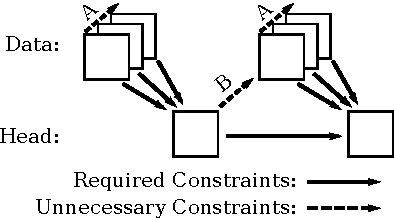
\includegraphics[width=.55\linewidth]{PersistencyModels/CWL_2LC_dependences.pdf}
  \caption{\textbf{Queue Persist Dependences.} Persist ordering dependences for \emph{Copy While Locked} and \emph{Two-Lock Concurrent}.  Constraints necessary for proper recovery shown as solid arrows; unnecessary constraints incurred by strict persistence appear as dashed arrows and are labelled as A (removed with epoch persistency) and B (further removed by strand persistency).}
  \label{fig::CWL_dependences}
\end{figure}


Both queue designs use the persistency model to prevent persists to the head pointer from occuring before persists to the data segment for each insert operation.
Algorithm~\ref{Alg::Queue} includes barriers for two different persistency models (described later in Section~\ref{section:PersistencyModels}).
Additionally, persist dependences (and unnecessary constraints introduced by strict persistency models) are shown in Figure~\ref{fig::CWL_dependences}.
Recovery requires that persists to the head pointer are ordered after persists to the data segment from the same insert operation and persists to the head pointer occur in insert-order to prevent holes in the queue.
All other persists within the same insert operation and between operations may be concurrent.
While not necessary for correct recovery, these persist dependences are difficult to describe minimally; ordering mechanisms often introduce unnecessary persist constraints (dashed lines in the Figure).

The previous designs trade off concurrency and complexity.
\emph{Copy While Locked}, while simple, serializes persists between insert operations.
On the other hand, \emph{Two-Lock Concurrent} allows greater concurrency, but requires two locks be acquired per insert and a volatile \emph{insert list} be maintained.
We consider a third design, \emph{Queue Holes}, that provides both improved persist concurrency and a high execution rate (first introduced in \cite{FangHsiao11}).

\begin{figure}
  \centering
  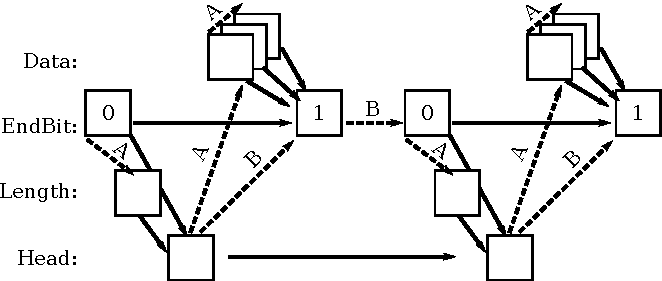
\includegraphics[width=\linewidth]{PersistencyModels/holes_dependences.pdf}
  \caption{\textbf{\emph{Queue Holes} Dependences.} The head pointer may not persist before \emph{endBit} and length; final \emph{endBit} may not persist until the entry persists to the data segment.  Strict persistency introduces several unnecessary constraints.}
  \label{fig::holes_dependences}
\end{figure}


\emph{Queue Holes} prepends each queue entry with its length and appends the entry with an endBit.
A single lock is held while reserving queue space and updating the head pointer, but is released prior to persisting the entry into the data segment.
An entry is recovered after failure if the entry is located within the region indicated by the head pointer (as in CWL and 2LC) and the entry's endBit is set.
The minimal set of persist dependences necessary for correct recovery are shown in Figure~\ref{fig::holes_dependences}.
The length and endBit persist before the head pointer; the data segment persists before setting the endBit; and persists to the same address occur in the order observed by cache coherence (endBits and the head pointer).
An inserted entry is recoverable only after the persist at line 37 completes, even though the head pointer is persisted earlier at line 33.

\section{Memory Persistency Models}
\label{sec:PersistencyModels:Models}

Section~\ref{section:Persistency} outlined potential classes of persistency models.
We now introduce several specific persistency models to be evaluated later in Section~\ref{section:Evaluation}.
All models assume SC as the underlying memory consistency model, and successively relax persistency to introduce specific optimizations.
For each model we discuss its motivation, give a definition, describe necessary annotations for and performance of our persistent queues, and offer possible implementations.

\subsection{Strict Persistency}
\label{section:PersistencyModels:Strict}

\textbf{Motivation.}
Our first persistency model is Strict Persistency, as discussed in Section~\ref{section:Persistency}.
Strict persistency simplifies reasoning about persist ordering by coupling persist dependences to the memory consistency model.
No additional persist barriers are required, easing the burden on the programmer.
While strict persistency provides an intuitive first model, under SC, it imposes persist ordering constraints that unnecessarily limit persist concurrency for many data structures, and requires programmers to resort to multi-threading to obtain concurrency.

\textbf{Definition.}
Under strict persistency, persist order observes all happens-before relations implied by execution's dynamic order of memory operations as viewed by the recovery observer.
Thus, all persists are ordered with respect to the program order of the issuing thread.
Note that, like store operations, persists from different threads that are unordered by happens-before (i.e., the recovery observer cannot distinguish which is first) are concurrent.

\textbf{Persist Performance.}
Strict persistency under SC introduces many unnecessary persist dependences.
Consequently, strict persistency must rely entirely on thread concurrency to enable concurrent persists.
Figures~\ref{fig::CWL_dependences} and~\ref{fig::holes_dependences} illustrate these unnecessary dependences and their causes.
Lacking mechanisms to relax persist ordering, strict persistency under SC introduces all the shown dependences (dashed lines).

\textbf{Implementation.}
A straight-forward implementation of strict persistency stalls issue of subsequent memory accesses until a store and its corresponding persist both complete.
Conventional speculation mechanisms may allow loads to speculatively reorder with respect to persistent stores \cite{Gharachorloo91}.
Buffered strict persistency can be implemented by serializing persists to a single, totally ordered queue in front of persistent memory (e.g., in a bus-based multiprocessor, persists can be queued after they are serialized by the bus).
Delays still occur when buffers fill or to drain the queue at persist sync instructions.

\subsection{Persist Epochs}
\label{section:PersistencyModels:PersistEpochs}

\textbf{Motivation.}
Strict persistency under SC introduces many persist dependences unnecessary for correct recovery.
The most common unnecessary persist dependence occurs due to the program-order constraint of SC.
A common programming pattern is to perform numerous persists to a large, contiguous region of memory that logically represents a single object, but which cannot occur atomically (due to their size).
Under strict persistency, the persists serialize.
We remove the program-order-implied persist order constraint with \emph{persist epochs}, allowing consecutive persists from the same thread to reorder and persist in parallel.
Doing so, however, requires annotation by the programmer in the form of persist barriers when ordering is required by the recovery algorithm.
Persist epochs additionally allow persists to addresses protected by a lock to reorder with respect to the lock operations (e.g., avoid delaying the lock release while the persist completes); our queue implementations leverage this optimization opportunity as well.

\textbf{Definition.}
Each thread's execution is separated into \emph{persist epochs} by persist barrier instructions.
Persist barriers enforce that no persist after the barrier may occur before any persist before the barrier.
Persists within each epoch (not separated by a barrier) are concurrent and may reorder or occur in parallel.
Memory operation visibility follows SC.

Additional complexity arises in reasoning about persist ordering across threads. 
We define a \emph{persist epoch race} as persist epochs from two or more threads that (1) include memory accesses (to volatile or persistent memory) that race, and (2) at least two of the epochs include persist operations. 
In the presence of persist epoch races, each persist barrier acts as a persist release for all persists prior to the barrier, and as a persist acquire for all accesses following the barrier \cite{Gharachorloo90}.
As a consequence, persists prior to the persist barrier immediately preceding the first access of the race are ordered before all persists after the next barrier following the second access of the race.
However, persists within the epochs participating in the persist epoch race are concurrent and may complete in parallel or out of order.

\textbf{Discussion.}
Barriers provide an intuitive mechanism to guarantee proper recovery as it is impossible at recovery to observe a persist from after a barrier while failing to observe a persist from before the same barrier.
However, many persists (those within the same epoch) are free to occur in parallel, improving persist concurrency.

As noted in our definition, reasoning about persist order across threads can be challenging.
Synchronization operations within persist epochs impose ordering across the store and load operations (due to SC memory ordering), but do not order corresponding persist operations.
Hence, persist operations correctly synchronized under SC by volatile locks may nevertheless result in astonishing persist ordering.
A simple (yet conservative) way to avoid persist epoch races is to place persist barriers before and after all lock acquires and releases.
The persist behavior of strict persistency can be achieved by preceding and following all persists with a persist barrier.

Persist epoch races may be intentionally introduced to increase persist concurrency; we discuss such an optimization below.
Enforcing persist order between threads with volatile locks requires that the persists be synchronized outside of the epochs in which the persists occur.
However, synchronization through persistent memory is possible.
Since persists to the same address must follow the order observed by cache coherence, even if they occur in epochs that race, the outcome of persist synchronization is well defined.
Hence, atomic read-modify-write operations to persistent memory addresses provide the expected behavior.

Our definition of persist epochs is inspired by the programming model and hardware extensions for caching persisent memory proposed for the Byte-addressable Persistent File System (BPFS) \cite{Condit09}.
However, we introduce several subtle differences that we believe make persist epochs a more intuitive model.
Our definition considers all memory accesses when determining persist ordering among threads, whereas the BPFS memory system orders persists only when conflicts occur to the persistent address space.
While the BPFS file system implementation avoids persist epoch races, it is not clear that the burden falls to the programmer to avoid such accesses or what persist behavior results when such races occur (we believe the BPFS authors' intent was to prohibit programs containing such races---the cache implementation deadlocks under persist epoch races containing circular persist dependences).  
Furthermore, BPFS detects conflicts to the persistent address space by recording the last thread and epoch to persist to each cache line; the next thread to access that line will detect the conflict.
Such an implementation, however, cannot detect conflicts where the first access is a load and the second a store.
As a result, BPFS detects conflicts to persistent memory according to TSO rather than SC ordering \cite{SPARCv9}.


\textbf{Persist Performance.}
Persist epochs remove all unnecessary persist dependences that resulted from strict persistency's program order constraint.
All versions of the persistent queue benefit from allowing persist entries to persist to the data segment concurrently, regardless of the size of the entry.
Additionally, \emph{Queue Holes} allows entry length and \emph{endBit} to persist concurrently (although both are ordered with respect to the subsequent persist of the head pointer).
Finally, many persist constraints between threads are removed by intentionally allowing persist epoch races.
\emph{Copy While Locked} and \emph{Queue Holes} retain recovery correctness by still ordering all persists to the head marker (persists will occur according to cache coherence order).
As a result, persists protected by a lock occur concurrently.

Algorithm~\ref{Alg::Queue} demonstrates how to use persist barriers (shown in the code as $PersistBarrier$) within our queue designs.
The constraints in Figures~\ref{fig::CWL_dependences} and~\ref{fig::holes_dependences} annotated with ``A" are removed under persist epochs relative to strict persistency.

\textbf{Implementation.}
BPFS \cite{Condit09} outlines cache extensions that provide a persistency model similar to persist epochs.
Modifications must be made to detect load-before-store conflicts (and thus enforce SC rather than TSO ordering) and track conflicts to volatile memory addresses as well as persistent memory addresses.
Instead of delaying execution to enforce persist ordering among threads, optimized implementations avoid stalling execution by buffering persists while recording and subsequently enforcing dependences among them, allowing persists to occur asynchronously despite access conflicts.

\subsection{Persist Strands}
\label{section:PersistencyModels:PersistStrands}

\textbf{Motivation.}
Persist epochs relax persist dependences within and across threads.
However, persists within a thread can only be labeled as concurrent if they are consecutive.
Likewise, persists from different threads are only concurrent if their epochs race or if they are not synchronized.
Many persists within and across threads may still correctly be made concurrent even if they do not fit these patterns.
We introduce \emph{persist strands}, a new persistency model to minimally annotate persist dependences.

\textbf{Definition.}
A strand is an interval of memory execution from a single thread.
Strands are separated via \emph{strand barriers}; each strand barrier begins a new strand.
The strand barrier clears all previously observed persist dependences from the executing thread.
Within each strand new and observed persists are ordered using persist barriers according to the persist epoch model.

\textbf{Discussion.}
There are no implicit persist ordering constraints across strands for persists to different addresses on the same thread of execution.
Ordering constraints arise only for persists to the same address as implied by cache coherence.
Hence, persists on a new strand may occur as early as possible and overlap with all preceding persists.
Persist strands allow programmers to indicate that logical tasks on the same thread are independent from the perspective of persistency.
To enforce necessary ordering, a persist strand begins by reading any memory locations after which new persists must be ordered.
These reads introduce an ordering dependency due to cache coherence, which can then be enforced with a subsequent epoch barrier.
This programming interface allows ordering constraints to be specified at the granularity of individual addresses.

\textbf{Persist Performance.}
Our persistent queue implementations place each insert task in a separate persist strand.
The result is that all unnecessary persist constraints are removed, including constraints between inserts from the same thread.
Algorithm~\ref{Alg::Queue} includes the necessary persist strand annotations ($NewStrand$ and $PersistBarrier$).
All unnecessary constraints from Figures~\ref{fig::CWL_dependences} and~\ref{fig::holes_dependences} are removed; those removed in moving from persist epochs to persist strands are labeled ``B."
The required persist dependences (and only those required for correct recovery) remain, maximizing persist concurrency.

\textbf{Implementation.}
Persist strands build on the hardware requirements to track persist dependencies as in persist epochs, but further require mechanisms to separate tracking of dependencies for different strands.  In addition to tracking the last thread to access each persistent location, the strand within the thread must also be tracked.  Unordered persists on different strands can traverse separate queues (e.g., on separate virtual channels) throughout the persistent memory system.  Persist strands give enormous implementation latitude and designing efficient hardware to track and observe only the minimal ordering requirements remains an open research challenge.  In this work, we focus on demonstrating the potential performance that the model allows. 

Relaxed persistency offers new tools to enforce recovery correctness while minimizing delays due to persists.
The next sections use these queue software designs and persistency models to quantitatively evaluate how much opportunity relaxed persistency holds to improve performance with NVRAM.
